\documentclass[12pt,letterpaper]{article}
\usepackage[utf8]{inputenc}
\usepackage[spanish]{babel}
\usepackage{graphicx}
\usepackage[left=2cm,right=2cm,top=2cm,bottom=2cm]{geometry}
\usepackage{graphicx} % figuras
% \usepackage{subfigure} % subfiguras
\usepackage{float} % para usar [H]
\usepackage{amsmath}
%\usepackage{txfonts}
\usepackage{stackrel} 
\usepackage{multirow}
\usepackage{enumerate} % enumerados
\renewcommand{\labelitemi}{$-$}
\renewcommand{\labelitemii}{$\cdot$}
% \author{}
% \title{Caratula}
\begin{document}

% Fancy Header and Footer
% \usepackage{fancyhdr}
% \pagestyle{fancy}
% \cfoot{}
% \rfoot{\thepage}
%

% \usepackage[hidelinks]{hyperref} % CREA HYPERVINCULOS EN INDICE

% \author{}
\title{Caratula}

\begin{titlepage}
\begin{center}
\large{UNERSIDAD PRIVADA DE TACNA}\\
\vspace*{-0.025in}
\begin{figure}[htb]
\begin{center}

\includegraphics[width=8cm]{./Imagenes/logo}
\end{center}
\end{figure}
\vspace*{0.15in}
INGENIERIA DE SISTEMAS  \\

\vspace*{0.5in}
\begin{large}
TITULO:\\
\end{large}

\vspace*{0.1in}
\begin{Large}
\textbf{INFORME DE LABORATORIO Nro 01} \\
\end{Large}

\vspace*{0.3in}
\begin{Large}
\textbf{CURSO:} \\
\end{Large}

\vspace*{0.1in}
\begin{large}
BASE DE DATOS II\\
\end{large}

\vspace*{0.3in}
\begin{Large}
\textbf{DOCENTE:} \\
\end{Large}

\vspace*{0.1in}
\begin{large}
 Ing. Patrick Cuadros Quiroga\\
\end{large}

\vspace*{0.2in}
\vspace*{0.1in}
\begin{large}
Integrantes: \\
\begin{flushleft}
Nilton Edy Perez Mamani		\hfill	(2015053233) \\
\end{flushleft}
\end{large}
\end{center}

\end{titlepage}


\tableofcontents % INDICE
\thispagestyle{empty} % INDICE SIN NUMERO
\newpage
\setcounter{page}{1} % REINICIAR CONTADOR DE PAGINAS DESPUES DEL INDICE

\section{Que es GitHub?} 

\begin{itemize}
GitHub es una plataforma de desarrollo colaborativo de software para alojar proyectos utilizando el sistema de control de versiones Git.

El código se almacena de forma pública, aunque también se puede hacer de forma privada, creando una cuenta de pago.
\end{itemize} 

\begin{center}

\includegraphics[width=10cm]{./Imagenes/github} 
\end{center}

\section{Para qué sirve?}
\begin{itemize}
GitHub aloja tu repositorio de código y te brinda herramientas muy útiles para el trabajo en equipo, dentro de un proyecto.
\end{itemize} 

\begin{center}

\includegraphics[width=10cm]{./Imagenes/herramienta} 
\end{center}

\begin{itemize}
Además de eso, puedes contribuir a mejorar el software de los demás. Para poder alcanzar esta meta, GitHub provee de funcionalidades para hacer un fork y solicitar pulls.
\end{itemize} 

\begin{center}

\includegraphics[width=10cm]{./Imagenes/herramienta2} 
\end{center}

\section{Qué herramientas proporciona?}
\begin{itemize}
En la actualidad, GitHub es mucho más que un servicio de alojamiento de código. Además de éste, se ofrecen varias herramientas útiles para el trabajo en equipo. Entre ellas, caben destacar:\\
\end{itemize} 

\begin{center}

\includegraphics[width=10cm]{./Imagenes/equipo} 
\end{center}

\begin{itemize}
a)Una wiki para el mantenimiento de las distintas versiones de las páginas.\\
b)Un sistema de seguimiento de problemas que permiten a los miembros de tu equipo detallar un problema con tu software o una sugerencia que deseen hacer.\\
c)Una herramienta de revisión de código, donde se pueden añadir anotaciones en cualquier punto de un fichero y debatir sobre determinados cambios realizados en un commit específico.\\
d)Un visor de ramas donde se pueden comparar los progresos realizados en las distintas ramas de nuestro repositorio.
\end{itemize}
\section{Qué uso le daremos?}
\begin{itemize}
En nuestra especialidad "Programación", fuimos aprendiendo cosas y creando programas de código abierto, fomentando el software libre; es por eso que presentamos esta gran herramienta enfocada al crecimiento de proyectos comunitarios y libres.\\
En esta página podremos crear una cuenta gratuita y comenzar a subir repositorios de código (o crearlos desde 0), para que con la ayuda de todos ese proyecto mejore; así como también fortalecer los proyectos de los demás para crecer como grupo.
\end{itemize}

\begin{center}

\includegraphics[width=10cm]{./Imagenes/proyecto} 
\end{center}

\section{Qué es Git?}
\begin{itemize}
Git es un sistema de control específico de versión de fuente abierta creada por Linus Torvalds en el 2005.\\
Específicamente, Git es un sistema de control de versión distribuida, lo que quiere decir que la base del código entero y su historial se encuentran disponibles en la computadora de todo desarrollador, lo cual permite un fácil acceso a las bifurcaciones y fusiones.
\end{itemize} 

\begin{center}

\includegraphics[width=10cm]{./Imagenes/git} 
\end{center}

\section{Necesidad de un control de versiones}
\begin{itemize}
El control de versiones es una de las tareas fundamentales para la administración de un proyecto de desarrollo de software en general. Surge de la necesidad de mantener y llevar control del código que vamos programando, conservando sus distintos estados. Es absolutamente necesario para el trabajo en equipo, pero resulta útil incluso a desarrolladores independientes.
\end{itemize}

\begin{itemize}
Para facilitarnos la vida existen sistemas como Git, Subversion, CVS, etc. que sirven para controlar las versiones de un software y que deberían ser una obligatoriedad en cualquier desarrollo. Nos ayudan en muchos ámbitos fundamentales, como podrían ser:\\

Comparar el código de un archivo, de modo que podamos ver las diferencias entre versiones\\
Restaurar versiones antiguas\\
Fusionar cambios entre distintas versiones\\
Trabajar con distintas ramas de un proyecto, por ejemplo la de producción y desarrollo\\
\end{itemize}

\section{Tipos de sistemas de control de versiones}
\begin{itemize}
Comenzaron a aparecer los sistemas de control del versionado del software allá por los años setenta, aunque al principio eran bastante elementales. Para hacerse una idea, en los primeros sistemas existía una restricción por la que sólo una persona podía estar a la vez tocando el mismo código. Es posible imaginarse que cosas semejantes provocaban retraso en los equipos de trabajo, por ello, a lo largo de los años fueron surgiendo nuevos sistemas de control de versiones, siempre evolucionando con el objetivo de resolver las necesidades de los equipos de desarrollo.
\end{itemize}

\begin{itemize}
\textbf{Sistemas de control de versiones locales}\\
Un método de control de versiones usado por mucha gente es copiar los archivos a otro directorio (quizás indicando la fecha y hora en que lo hicieron, si son avispados). Este enfoque es muy común porque es muy simple, pero también tremendamente propenso a errores. Es fácil olvidar en qué directorio te encuentras, y guardar accidentalmente en el archivo equivocado o sobrescribir archivos que no querías.\\

Para hacer frente a este problema, los programadores desarrollaron hace tiempo VCSs locales que contenían una simple base de datos en la que se llevaba registro de todos los cambios realizados sobre los archivos.
\end{itemize}

\begin{center}
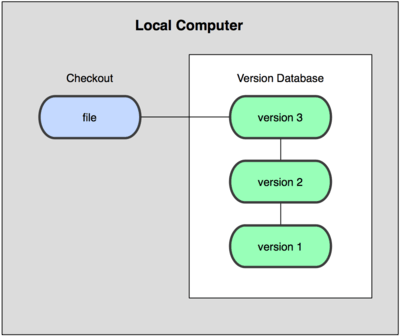
\includegraphics[width=10cm]{./Imagenes/local} 
\end{center}

\begin{itemize}
\textbf{Sistemas de control de versiones centralizados}\\
En estos sistemas hay un servidor que mantiene el repositorio y en el que cada programador mantiene en local únicamente aquellos archivos con los que está trabajando en un momento dado. Yo necesito conectarme con el servidor donde está el código para poder trabajar y enviar cambios en el software que se está programando. Ese sistema centralizado es el único lugar donde está todo el código del proyecto de manera completa. Subversion o CVS son sistemas de control de versiones centralizados.
\end{itemize}

\begin{center}
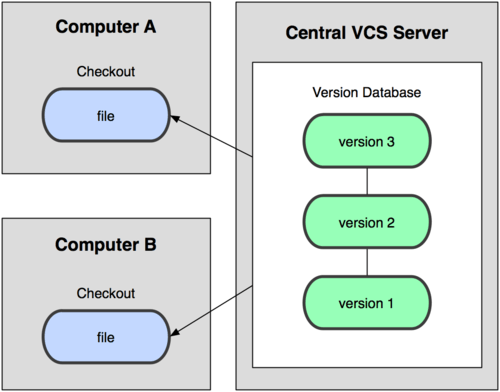
\includegraphics[width=10cm]{./Imagenes/centralizado} 
\end{center}

\begin{itemize}
\textbf{Sistemas de control de versiones distribuidos}\\
En este tipo de sistemas cada uno de los integrantes del equipo mantiene una copia local del repositorio completo. Al disponer de un repositorio local, puedo hacer commit (enviar cambios al sistema de control de versiones) en local, sin necesidad de estar conectado a Internet o cualquier otra red. En cualquier momento y en cualquier sitio donde esté puedo hacer un commit. Es cierto que es local de momento, luego podrás compartirlo con otras personas, pero el hecho de tener un repositorio completo me facilita ser autónomo y poder trabajar en cualquier situación. Git es un sistema de control de versiones distribuido.
\end{itemize}

\begin{center}
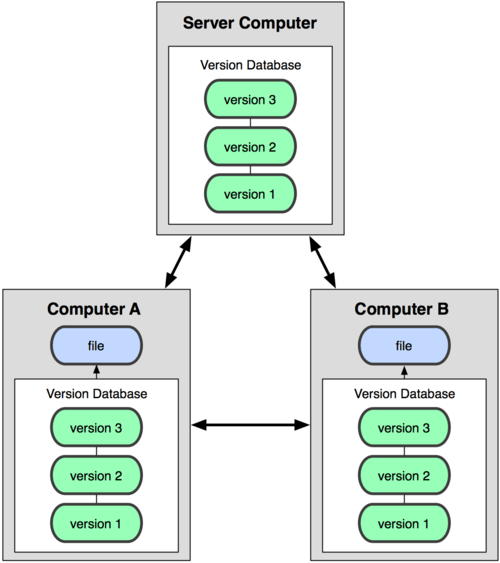
\includegraphics[width=10cm]{./Imagenes/distribuido} 
\end{center}


\end{document}
